\section{Empty-state latency and a carrier-funded activity witness}\label{sec:activity}
Finite energy and a matched work account permit activity, but neither forces it for every preparation. This section first proves a latency bound for arbitrary RX preparation with empty added states. It then chooses one preparation for which both strict receiving and a later nonzero incoming return can be proved. The two conclusions concern different quantities.

\subsection{What emptiness delays}
\begin{proposition}[Latency]\label{prop:latency}
If $u_{+,0}=u_{-,0}=0$ and $\zeta_0=0$, then for arbitrary finite-energy RX preparation,
\begin{equation}\label{eq:latency}
H_G(t)=0\quad(0\le t\le\theta_-),\qquad
b(t)=0\quad\textnormal{a.e. on }[0,2\theta_-).
\end{equation}
\end{proposition}
\begin{proof}
Before $\theta_-$, the forward characteristic has not crossed any interval. Its initial-profile part is zero, so c is zero a.e. The receiving variation-of-constants formula with zero initial data gives $\zeta=0$, hence d is zero there. Before $2\theta_-$, b is either its zero initial-profile part or d at $t-\theta_X(s)<\theta_-$; this is again zero. Continuity of $\zeta$ includes the endpoint $t=\theta_-$ in the stock statement. No instantaneous trace value at either onset is needed.
\end{proof}
Thus the incoming force $\sqrt2\kappa J^*b$ is delayed, while the term $-\kappa^2Q$ acts immediately to launch the forward field. The result does not say that either stock or boundary trace must become nonzero at its threshold.

\subsection{A preparation with strict receiving}
Fix $\kappa>0$ and prepare
\begin{equation}\label{eq:preload}
x_0=0,\quad z_0=0,\quad Q_0(s)=(P,0),\quad P>0,\qquad
u_{+,0}=u_{-,0}=0,\quad\zeta_0=0.
\end{equation}
Since $f(0)=J_f(0)=0$, uniqueness keeps x identically zero during exchange. Old z continues to obey its retained equation; it is not clamped to zero. Before $2\theta_-$ there is no incoming b, and the carrier satisfies
\begin{equation}\label{eq:earlycarrier}
Q(t)=e^{-\kappa^2t}S_c(t)Q_0+
\int_0^t e^{-\kappa^2(t-v)}S_c(t-v)(\Bcal q(v),0)\dd v.
\end{equation}
The finite-width profiles are H1 and q is continuous, so the integral is continuous into $H^1_{\rm per}$ on every closed interval before $2\theta_-$. The one-dimensional periodic embedding $H^1\hookrightarrow C^0$ and continuity at the constant initial state give some $0<\varepsilon<\theta_-$ such that
\begin{equation}\label{eq:earlypositive}
p(s,u)>P/2,\qquad |Q(s,u)|\le2P
\quad(s\in S_L,\ 0\le u\le\varepsilon).
\end{equation}
This temporary regularity follows from this preparation and equation, not from the energy bound alone. Zero initial line profiles and a nonzero boundary launch at zero are permitted in the mild solution class; no corner compatibility or later global H1 claim is introduced.

\begin{proposition}[Strict receiving from carrier preload]\label{prop:receiving}
For~\eqref{eq:preload} and sufficiently small $\varepsilon>0$ as above,
\begin{equation}\label{eq:strictreceiving}
0<H_G(t)\le LP^2/2\qquad
(\theta_-<t<\theta_-+\varepsilon).
\end{equation}
\end{proposition}
\begin{proof}
Every arrival in this interval samples a near time in $[0,\varepsilon)$, where b is zero. Hence $c=\sqrt2\kappa\ii_{t\ge\theta}JQ(t-\theta)$. The scalar block of the Gram matrix decouples from the vector block and gives
\begin{equation}\label{eq:scalarreceiving}
\beta_G\partial_t\zeta_{\rm sc}(X,t)+m_0(X)\zeta_{\rm sc}(X,t)
=2\kappa a_o\int_{\theta_X(s)\le t}\frac{p(s,t-\theta_X(s))}{d_X(s)}\dd s\ge0.
\end{equation}
Its integrating-factor formula, starting from zero, proves nonnegativity. For strict positivity at any fixed $t\in(\theta_-,\theta_-+\varepsilon)$, choose $\theta_-<r<t$. A minimizing pair for the continuous delay exists on the compact labeled geometry. A relative product neighborhood has $\theta<r$. If its G point is a tip or elbow, move into an adjacent segment interior while preserving the strict inequality. Shrink to a circle interval I and an interior G interval J of positive arclength with $\sup_{I\times J}\theta<r$.

For $X\in J$ and $v\in[r,t]$, the I contribution to the right side of~\eqref{eq:scalarreceiving} is at least $\kappa a_oP|I|/(c_e\theta_+)$. Consequently
\begin{equation}\label{eq:strictlower}
\zeta_{\rm sc}(X,t)\ge
\frac{\kappa a_oP|I|}{\beta_Gc_e\theta_+}
\int_r^t e^{-m_0(X)(t-v)/\beta_G}\dd v>0
\quad\textnormal{for a.e. }X\in J.
\end{equation}
Positive arclength of J gives $H_G(t)>0$. This argument works for every t strictly above the minimum; it requires neither delay differentiation nor an interior minimizer. Since $\zeta$ is continuous in Y, the all-times stock assertion is meaningful. Conservation bounds it by the initial total stock $LP^2/2$.
\end{proof}
The witness is funded by the declared carrier preload. It establishes no native empty-launch receiving, recovery, capacity fraction, or equal and simultaneous activity at all six labels.

\subsection{A later nonzero incoming return}
\begin{proposition}[Incoming boundary activity]\label{prop:return}
The same preparation admits a further reduction of $\varepsilon$ such that
\begin{equation}\label{eq:returnnonzero}
\norm{b(t)}_V>0\quad\textnormal{for a.e. }t\in(2\theta_-,2\theta_-+\varepsilon).
\end{equation}
\end{proposition}
\begin{proof}
The early formula for c, $|A_sQ|=|Q|$, and~\eqref{eq:earlypositive} give
\begin{equation}\label{eq:earlyCbound}
\norm{Cc(v)}_{L^\infty(G)}\le\frac{2\sqrt2\kappa a_oPL}{\delta_w}
\quad(\theta_-\le v\le\theta_-+\varepsilon).
\end{equation}
The positive semidefinite pointwise matrix $\Gmat(X)$ has a contraction exponential. Its receiving formula therefore supplies a representative with
\begin{equation}\label{eq:earlyzetabound}
\norm{\zeta(v)}_{L^\infty(G)}\le
\frac{4\kappa a_oPL}{\beta_G\delta_w}(v-\theta_-).
\end{equation}
This bound uses the bounded early forcing of this witness; it is not an L-infinity theorem for arbitrary energy preparations. Shrink $\varepsilon$ without losing~\eqref{eq:earlypositive} so that
\begin{equation}\label{eq:epsreturn}
\varepsilon<\frac{\beta_G\delta_w^2}{16a_o^2ML}.
\end{equation}
For $2\theta_-<t<2\theta_-+\varepsilon$ and a channel with $\theta=\theta_X(s)<t/2$, set $v=t-\theta$ and $u=t-2\theta$. Then $\theta_-<v<\theta_-+\varepsilon$ and $0<u<\varepsilon$. Its scalar arrival and far effort obey
\begin{align}
c_p(s,X,v)&=\frac{\sqrt2\kappa}{\sqrt M}p(s,u)>
\frac{\kappa P}{\sqrt{2M}},\notag\\
\abs{\sqrt2(C^*\zeta(v))_p(s,X)}&\le
\frac{4\sqrt2\kappa a_o^2P\sqrt M L}{\beta_G\delta_w^2}\varepsilon
<\frac{\kappa P}{2\sqrt{2M}}.\label{eq:effortbound}
\end{align}
The far law and backward characteristic now yield
\begin{equation}\label{eq:negativeb}
b_p(s,X,t)=d_p(s,X,t-\theta)<-\frac{\kappa P}{2\sqrt{2M}}<0
\quad\textnormal{on }\{\theta_X(s)<t/2\}.
\end{equation}
The same relative-neighborhood argument used in the receiving proof gives this sublevel set positive product measure for every $t>2\theta_-$. Thus the L2 trace is nonzero for a.e. t in the asserted interval. The bounded early carrier and pointwise receiving formulas also define a characteristic representative for which the inequality holds at every such t. The energy-space conclusion needs no particular representative at a single onset time.
\end{proof}
The constant 16 in~\eqref{eq:epsreturn} makes the effort bound strictly less than half the direct lower bound. Nonzero b is distinct from $J^*b\ne0$, positive net carrier work, native credit and recovery. Projection and simultaneous launch still enter the actual force. Figure~\ref{fig:time} separates these latency results from the temporal-adjoint support of Section~\ref{sec:observation}.

\begin{figure}[tbp]\centering
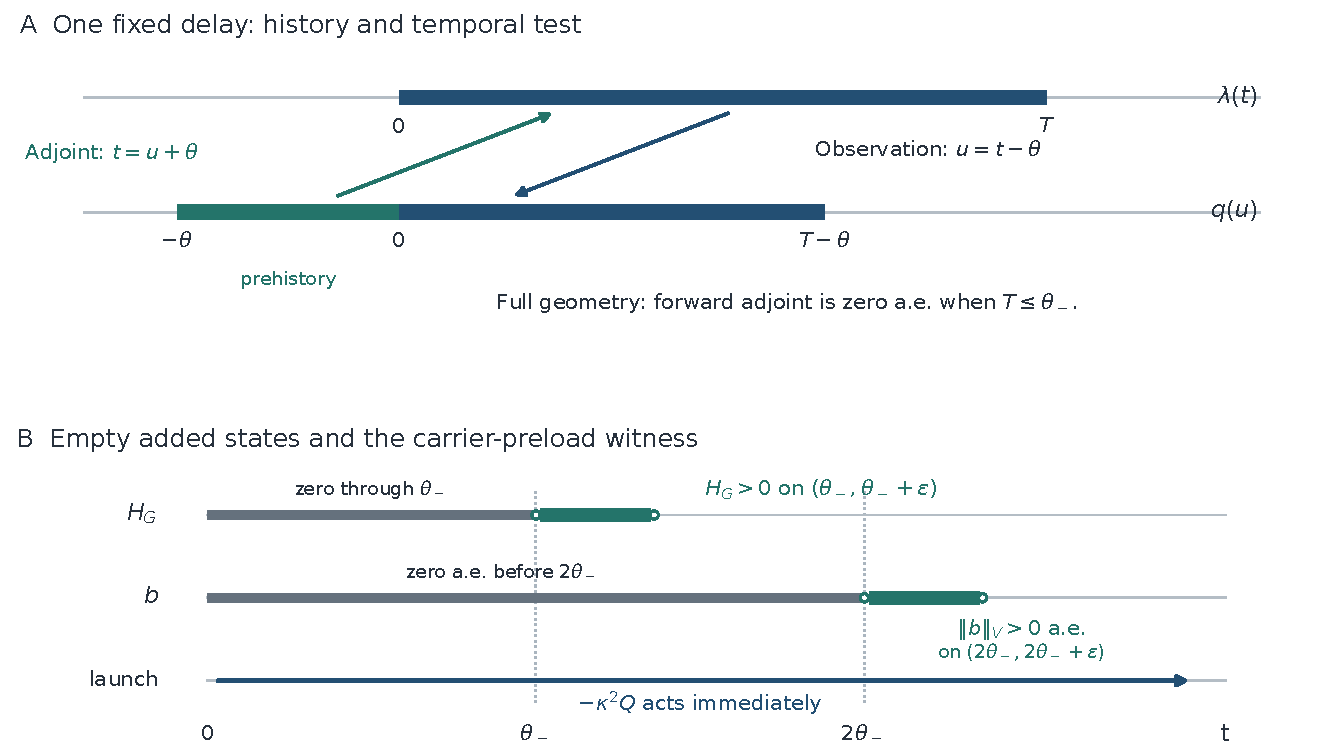
\includegraphics[width=\textwidth]{figures/time_support.pdf}
\caption{Two different time accounts. Top: for one fixed delay, causal observation reads earlier carrier data, while the finite-window temporal adjoint evaluates a later test time and has a prehistory part. Bottom: empty added states impose the proven latency bounds; the constant carrier-preload witness gives strict receiving and a nonzero incoming boundary trace on short open intervals. Interval lengths and positions are schematic. These are supports and bounds, not simulated waveforms or exact onset amplitudes.}\label{fig:time}
\end{figure}
